\documentclass[10pt]{article}
\usepackage[letterpaper]{geometry}
\geometry{verbose,tmargin=1in,bmargin=1in,lmargin=1in,rmargin=1in}
\usepackage{setspace}
\usepackage{ragged2e}
\usepackage{color}
\usepackage{titlesec}
\usepackage{graphicx}
\usepackage{float}
\usepackage{mathtools}
\usepackage{amsmath}
\usepackage[font=small,labelfont=bf,labelsep=period]{caption}
\usepackage[english]{babel}
\usepackage{indentfirst}
\usepackage{array}
\usepackage{makecell}
\usepackage[usenames,dvipsnames]{xcolor}
\usepackage{multirow}
\usepackage{tabularx}
\usepackage{arydshln}
\usepackage{caption}
\usepackage{subcaption}
\usepackage{xfrac}
\usepackage{etoolbox}
\usepackage{cite}
\usepackage{url}
\usepackage{dcolumn}
\usepackage{hyperref}
\usepackage{courier}
\usepackage{url}
\usepackage{esvect}
\usepackage{commath}
\usepackage{verbatim} % for block comments
\usepackage{enumitem}
\usepackage{hyperref} % for clickable table of contents
\usepackage{braket}
\usepackage{titlesec}
\usepackage{booktabs}
\usepackage{gensymb}
\usepackage{longtable}
\usepackage{listings}
\lstset{
    frame=single,
    breaklines=true,
    postbreak=\raisebox{0ex}[0ex][0ex]{\ensuremath{\color{red}\hookrightarrow\space}}
}

% for circled numbers
\usepackage{tikz}
\newcommand*\circled[1]{\tikz[baseline=(char.base)]{
            \node[shape=circle,draw,inner sep=2pt] (char) {#1};}}


\titleclass{\subsubsubsection}{straight}[\subsection]

% define new command for triple sub sections
\newcounter{subsubsubsection}[subsubsection]
\renewcommand\thesubsubsubsection{\thesubsubsection.\arabic{subsubsubsection}}
\renewcommand\theparagraph{\thesubsubsubsection.\arabic{paragraph}} % optional; useful if paragraphs are to be numbered

\titleformat{\subsubsubsection}
  {\normalfont\normalsize\bfseries}{\thesubsubsubsection}{1em}{}
\titlespacing*{\subsubsubsection}
{0pt}{3.25ex plus 1ex minus .2ex}{1.5ex plus .2ex}

\makeatletter
\renewcommand\paragraph{\@startsection{paragraph}{5}{\z@}%
  {3.25ex \@plus1ex \@minus.2ex}%
  {-1em}%
  {\normalfont\normalsize\bfseries}}
\renewcommand\subparagraph{\@startsection{subparagraph}{6}{\parindent}%
  {3.25ex \@plus1ex \@minus .2ex}%
  {-1em}%
  {\normalfont\normalsize\bfseries}}
\def\toclevel@subsubsubsection{4}
\def\toclevel@paragraph{5}
\def\toclevel@paragraph{6}
\def\l@subsubsubsection{\@dottedtocline{4}{7em}{4em}}
\def\l@paragraph{\@dottedtocline{5}{10em}{5em}}
\def\l@subparagraph{\@dottedtocline{6}{14em}{6em}}
\makeatother

\newcommand{\volume}{\mathop{\ooalign{\hfil$V$\hfil\cr\kern0.08em--\hfil\cr}}\nolimits}

\setcounter{secnumdepth}{4}
\setcounter{tocdepth}{4}
\begin{document}

\title{ME 280a: HW 1}
\author{April Novak}

\maketitle

\section{Introduction and Objectives}

The purpose of this study is to solve a simple finite element (FE) problem and perform a convergence study to determine the number of elements needed to reach a particular error relative to an analytical solution. The Galerkin FE method is used, which for certain classes of problems possesses the ``best approximation property,'' a characteristic that signifies that the FE solution obtained is the best possible solution for a given mesh refinement and choice of shape functions. The mathematical procedure and numerical implementation is described in Section \ref{sec:Procedure}.

\section{Procedure}
\label{sec:Procedure}

This section details the problem statement and mathematical method used for solving the problem.

\subsection{Problem Statement}

This section describes the mathematical process used to solve the following problem:

\begin{equation}
\label{eq:Problem}
\frac{d}{dx}\left(E(x)\frac{du}{dx}\right)=k^2\sin{\left(\frac{2\pi kx}{L}\right)}
\end{equation}

where \(E\) is the modulus of elasticity, \(u\) is the solution, \(k\) is a known constant, \(L\) is the problem domain length, and \(x\) is the spatial variable. In order to verify that the program functions correctly, the FE solution to Eq. \eqref{eq:Problem} will be compared with the analytical solution to Eq. \eqref{eq:Problem}. To determine the analytical solution, integrate Eq. \eqref{eq:Problem} once to obtain:

\begin{equation}
\label{eq:Problem2}
\frac{du}{dx}=-\frac{1}{E}k^2\cos{\left(\frac{2\pi kx}{L}\right)}\frac{L}{2\pi k}+C_1
\end{equation}

It has been assumed that \(E\) is not a function of \(x\), and hence can be treated as constant in the integration. Integrating once more:

\begin{equation}
\label{eq:Problem2}
u(x)=-\frac{1}{E}k^2\sin{\left(\frac{2\pi kx}{L}\right)}\left(\frac{L}{2\pi k}\right)^2+C_1x+C_2
\end{equation}

The boundary conditions for this problem are Dirichlet at both endpoints, such that:

\begin{equation}
\begin{aligned}
u(0)=0\\
u(L)=1\\
\end{aligned}
\end{equation}

By the first BC, \(C_2=0\), and \(C_1\) based on the second condition equals:

\begin{equation}
C_1=\frac{u(L)+k^2\sin{(2\pi k)}\left(\frac{L}{2\pi k E}\right)^2}{L}
\end{equation}

The purpose of this assignment is to solve Eq. \eqref{eq:Problem} with the finite element method (FEM) and then to determine how many elements are needed to obtain a specified error as a function of the frequency \(k\). The solutions for various numbers of elements will also be compared to illustrate how increasing the number of elements ``hones in'' on the analytical solution.

\subsection{Finite Element Implementation}

The Galerkin FEM achieves the best approximation property by approximating the true solution \(u(x)\) as \(u^N(x)\), where both \(u^N(x)\) and the test function \(\psi\) are expanded in the same set of \(N\) basis functions \(\phi\):

\begin{equation}
\label{eq:approx}
\begin{aligned}
u\approx u^N=\sum_{j=1}^{N}a_j\phi_j\\
\psi=\sum_{i=1}^{N}b_i\phi_i\\
\end{aligned}
\end{equation}

Galerkin's method is stated as:

\begin{equation}
r^N\cdot u^N=0
\end{equation}

where \(r^N\) is the residual. Hence, to formulate the weak form to Eq. \eqref{eq:Problem}, multiply Eq. \eqref{eq:Problem} through by \(\psi\) and integrate over all space, \(d\Omega\).

\begin{equation}
\int_{\Omega}^{}\frac{d}{dx}\left(E(x)\frac{du}{dx}\right)\psi d\Omega-\int_{\Omega}^{}k^2\sin{\left(\frac{2\pi kx}{L}\right)}\psi d\Omega=0
\end{equation}

Applying integration by parts to the first term:

\begin{equation}
-\int_{\Omega}^{}E(x)\frac{du}{dx}\frac{d\psi}{dx}d\Omega+\int_{\partial\Omega}^{}E(x)\frac{du}{dx}\psi d(\partial\Omega)-\int_{\Omega}^{}k^2\sin{\left(\frac{2\pi kx}{L}\right)}\psi d\Omega=0
\end{equation}

where \(\partial\Omega\) refers to one dimension lower than \(\Omega\), which for this case refers to evaluation at the endpoints of the domain. Hence, for this particular 1-D problem, the above reduces to:

\begin{equation}
\begin{aligned}
-\int_{0}^{L}E(x)\frac{du}{dx}\frac{d\psi}{dx}dx+ E(x)\frac{du}{dx}\psi\biggr\vert_{0}^{L}-\int_{0}^{L}k^2\sin{\left(\frac{2\pi kx}{L}\right)}\psi dx=0\\
\int_{0}^{L}E(x)\frac{du}{dx}\frac{d\psi}{dx}dx=-\int_{0}^{L}k^2\sin{\left(\frac{2\pi kx}{L}\right)}\psi dx+E(x)\frac{du}{dx}\psi\biggr\vert_{0}^{L}\\
\end{aligned}
\end{equation}

Inserting the approximation described in Eq. \eqref{eq:approx}:

\begin{equation}
\begin{aligned}
\int_{0}^{L}E(x)\frac{d\left(\sum_{j=1}^{N}a_j\phi_j\right)}{dx}\frac{d\left(\sum_{i=1}^{N}b_i\phi_i\right)}{dx}dx=-\int_{0}^{L}k^2\sin{\left(\frac{2\pi kx}{L}\right)}\sum_{i=1}^{N}b_i\phi_idx+E(x)\frac{du}{dx}\sum_{i=1}^{N}b_i\phi_i\biggr\vert_{0}^{L}\\
\end{aligned}
\end{equation}

Recognizing that \(b_i\) appears in each term, the sum of the remaining terms must also equal zero (i.e. basically cancel \(b_i\) from each term).

\begin{equation}
\begin{aligned}
\int_{0}^{L}E(x)\frac{d\left(\sum_{j=1}^{N}a_j\phi_j\right)}{dx}\frac{d\phi_i}{dx}dx=-\int_{0}^{L}k^2\sin{\left(\frac{2\pi kx}{L}\right)}\phi_idx+E(x)\frac{du}{dx}\phi_i\biggr\vert_{0}^{L}\\
\end{aligned}
\end{equation}

This equation can be satisfied for each choice of \(j\), and hence can be reduced to:

\begin{equation}
\begin{aligned}
\int_{0}^{L}E(x)\frac{d\left(a_j\phi_j\right)}{dx}\frac{d\phi_i}{dx}dx=-\int_{0}^{L}k^2\sin{\left(\frac{2\pi kx}{L}\right)}\phi_idx+E(x)\frac{du}{dx}\phi_i\biggr\vert_{0}^{L}\\
\end{aligned}
\end{equation}

This produces a system of matrix equations of the form:

\begin{equation}
\label{eq:MatrixEqn}
\textbf{K}\vv{a}=\vv{F}
\end{equation}

where:

\begin{equation}
\begin{aligned}
\label{eq:SystemEquations}
K_{ij}=\int_{0}^{L}E(x)\frac{d\phi_i}{dx}\frac{d\phi_j}{dx}dx\\
a_j=a_j\\
F_i=-\int_{0}^{L}k^2\sin{\left(\frac{2\pi kx}{L}\right)}\phi_idx+E(x)\frac{du}{dx}\phi_i\biggr\vert_{0}^{L}\\
\end{aligned}
\end{equation}

where the second term in \(F_i\) is only applied at nodes that have Neumann boundary conditions (since \(\psi\) satisfies the homogeneous form of the essential boundary conditions). The above equation governs the entire domain. \(\textbf{K}\) is an \(n \times n\) matrix, where \(n\) is the number of global nodes. The solution is contained within \(\vv{a}\). This matrix system is solved in this assignment by simple Gaussian elimination, such that \(\vv{a}=\textbf{K}^{-1}\vv{F}\).

Quadrature is used to perform the numerical integration because it is much faster, and more general, than symbolic integration of the terms appearing in Eq. \eqref{eq:SystemEquations}. In order for these equations to be useful with Gaussian quadrature, they must be transformed to the master element which exists over \(-1\leq\xi\leq1\):

\begin{equation}
\begin{aligned}
K_{ij}=\int_{0}^{L}E(x)\frac{d\phi_i}{dx}\frac{d\phi_j}{dx}dx\rightarrow\int_{-1}^{1}E(x(\xi))\frac{d\phi_i}{dx}\frac{d\phi_j}{dx}dx\left(\frac{dx}{d\xi}\frac{dx}{d\xi}\frac{d\xi}{dx}\right)\rightarrow\int_{-1}^{1}E(x(\xi))\frac{d\phi_i}{d\xi}\frac{d\phi_j}{d\xi}dx\left(\frac{d\xi}{dx}\right)\\
a_j=a_j\\
F_i=-\int_{0}^{L}k^2\sin{\left(\frac{2\pi kx}{L}\right)}\phi_idx\rightarrow-\int_{-1}^{1}k^2\sin{\left(\frac{2\pi kx(\xi)}{L}\right)}\phi_i\frac{dx}{d\xi}d\xi\\
\end{aligned}
\end{equation} 

where the second term in \(F_i\) has been dropped because there are no Neumann boundary conditions in this assignment. For linear elements, the shape functions have the following form over the master element:

\begin{equation}
\begin{aligned}
\phi_1(\xi)=\frac{1-\xi}{2}\\
\phi_2(\xi)=\frac{1+\xi}{2}\\
\end{aligned}
\end{equation}

And the derivative of these functions with respect to the isoparametric coordinate are:

\begin{equation}
\begin{aligned}
\frac{d\phi_1(\xi)}{d\xi}=-1/2\\
\frac{d\phi_2(\xi)}{d\xi}=1/2\\
\end{aligned}
\end{equation}

The transformation from the physical domain (\(x\)) to the parent domain (\(\xi\)) is done with an isoparametric mapping:

\begin{equation}
\label{eq:Mapping}
x(\xi)=\sum_{i=1}^{N} X_i\phi_i(\xi)
\end{equation}

where \(X_i\) are the coordinates in each element. This mapping is performed for each element individually. The Jacobian \(dx/d\xi\) is obtain from Eq. \eqref{eq:Mapping} by differentiation:

\begin{equation}
\frac{dx(\xi)}{d\xi}=\sum_{i=1}^{N} X_i\frac{d\phi_i(\xi)}{d\xi}
\end{equation}

With all these transformations from the physical domain to the isoparametric domain, Gaussian quadrature can be used. For simplicity, a two-point quadrature rule is used, with the following weights \(w\) and sampling points \(x\):

\begin{equation}
\begin{aligned}
w=[1.0, 1.0]\\
x=[-\sqrt{1/3}, \sqrt{1/3}]\\
\end{aligned}
\end{equation} 

Transformation to the isoparametric domain therefore easily allows construction of the local stiffness matrix and local force matrix. The actual numerical algorithm computes the elemental \(k(i,j)\) and \(b(i)\) by looping over \(i, j\), and the quadrature points. Because each calculation is computed over a single element, a connectivity matrix is used to populate the global stiffness matrix and the global forcing vector with the elemental matrices and vectors. See the Appendix for the full code used in this assignment. After the global matrix and vector are formed, the global matrix has a banded-diagonal structure. 

In order to apply the boundary conditions within the numerical context of the finite element method, the matrix equation in Eq. \eqref{eq:MatrixEqn} must be rewritten to reflect that some of the nodal values are actually already specified through the Dirichlet boundary conditions. 

\begin{equation}
\label{eq:condensation}
\begin{bmatrix}
	K_{kk} & K_{ku}\\
	K_{uk} & K_{uu}\\
\end{bmatrix}
\begin{bmatrix}
	x_k\\
	x_u\\
\end{bmatrix}
=
\begin{bmatrix}
	F_k\\
	F_u\\
\end{bmatrix}
\end{equation}

where \(k\) indicates a known quantity (specified through a boundary condition) and \(u\) indicates an unknown quantity.   Explicitly expanding this equation gives:

\begin{equation}
\begin{aligned}
K_{kk}x_k+K_{ku}x_u=F_k\\
K_{uk}x_k+K_{uu}x_u=F_u\\
\end{aligned}
\end{equation}

Solving this matrix system is sometimes referred to as ``static condensation,'' since the original matrix system in Eq. \eqref{eq:MatrixEqn} must be separated into its components. The nodes at which Dirichlet conditions are specified are ``known,'' while all other nodes, including Neumann condition nodes, are ``unknown,'' since it is the value of \(u\) that we are looking to find at each node. The second of these equations is the one that is solved in this assignment, since there are no natural boundary conditions.

Once the solution is obtained by simple Gaussian elimination, the solution is transformed back to the physical domain (from the isoparametric domain) by solving a linear matrix system to determine the coefficients on the basis functions over each element (in the physical domain). For example, for a quadratic shape function, over one element with coordinates \(x_1, x_2,\) and \(x_3\), with solution values \(a_1, a_2,\) and \(a_3\), the following linear system solves for the coordinates on the shape function in the physical domain, in that element:

\begin{equation}
\label{eq:LinearSolve}
\begin{bmatrix}
1 & x_1 & x_1^2\\
1 & x_2 & x_2^2\\
1 & x_3 & x_3^2\\
\end{bmatrix}
\begin{bmatrix} A\\ B\\ C
\end{bmatrix}
=
\begin{bmatrix} a_1 \\ a_2 \\ a_3
\end{bmatrix}
\end{equation}

Each element is looped over to obtain the coefficients on the shape functions in the physical domain. This then transforms the solution back to the physical domain, and completes the FE solution.

\subsection{Error Estimates and Convergence Criteria}

The accuracy of the FE solution is estimated using the energy norm \(e^N\), defined as:

\begin{equation}
e^N=\frac{\|u-u^N\|}{\|u\|}
\end{equation}

where:

\begin{equation}
\|u\|=\sqrt{\int_{\Omega}^{}\frac{du}{dx}E\frac{du}{dx}}
\end{equation}

\begin{equation}
\|u-u^N\|=\sqrt{\int_{\Omega}^{}\frac{d(u-u^N)}{dx}E\frac{d(u-u^N)}{dx}}=\sqrt{\int_{\Omega}^{}\left(\frac{du}{dx}-\frac{du^N}{dx}\right)E\left(\frac{du}{dx}-\frac{du^N}{dx}\right)}
\end{equation}

The derivatives of the FE solution are determined according to:

\begin{equation}
\frac{du^N}{dx}=\frac{d}{dx}\sum_{j=1}^{N}a_j\phi_j(x)=\sum_{j=1}^{N}a_j\frac{d\phi_j(x)}{dx}=\sum_{j=1}^{N}a_j\frac{d\phi_j(x)}{d\xi}\frac{d\xi}{dx}
\end{equation}

while the derivative of the analytical solution is obtained from Eq. \eqref{eq:Problem2}. Convergence is defined to have been achieved for a given \(k\) and number of elements \(N\) once:

\begin{equation}
\label{eq:Convergence}
e^N=\frac{\|u-u^N\|}{\|u\|} \leq 0.05
\end{equation}

\subsection{Solution Results and Discussion}

Table \ref{table:N} shows the number of elements needed to satisfy Eq. \eqref{eq:Convergence} for each \(k\).

\begin{table}[H]
\caption{Number of elements \(N\) needed to reach convergence according to Eq. \eqref{eq:Convergence}.}
\centering
\begin{tabular}{l c}
\hline\hline
k & \(N\) to reach convergence\\ [0.5ex]
\hline
1 & 28\\
2 & 67\\
4 & 142\\
8 & 289\\
16 & 580\\
32 & 1160\\
\hline
\end{tabular}
\label{table:N}
\end{table}

Fig. \ref{Nplots} shows the FE solutions for \(N=2, 4, 8, 16, 32, 64, \) and \(128\) for \(k=1, 2, 4, 8, 16, 32\). The exact solution is also plotted for comparison. As can be seen, in general, increasing \(N\) improves the finite element solution with respect to better-approximating the analytical solution. It is interesting to note that, for choices of the number of elements \(N\) that are twice the value of \(k\) (i.e. for \(N=2k\)), the finite element solution is a straight line between the two endpoints. This likely occurs because of the highly oscillatory nature of the analytical solution, and the fact that too-few elements fails to place nodes at locations that represent the peaks and valleys of the analytical solution.

\begin{figure}[H]
\centering
\begin{subfigure}{.48\textwidth}
  \centering
  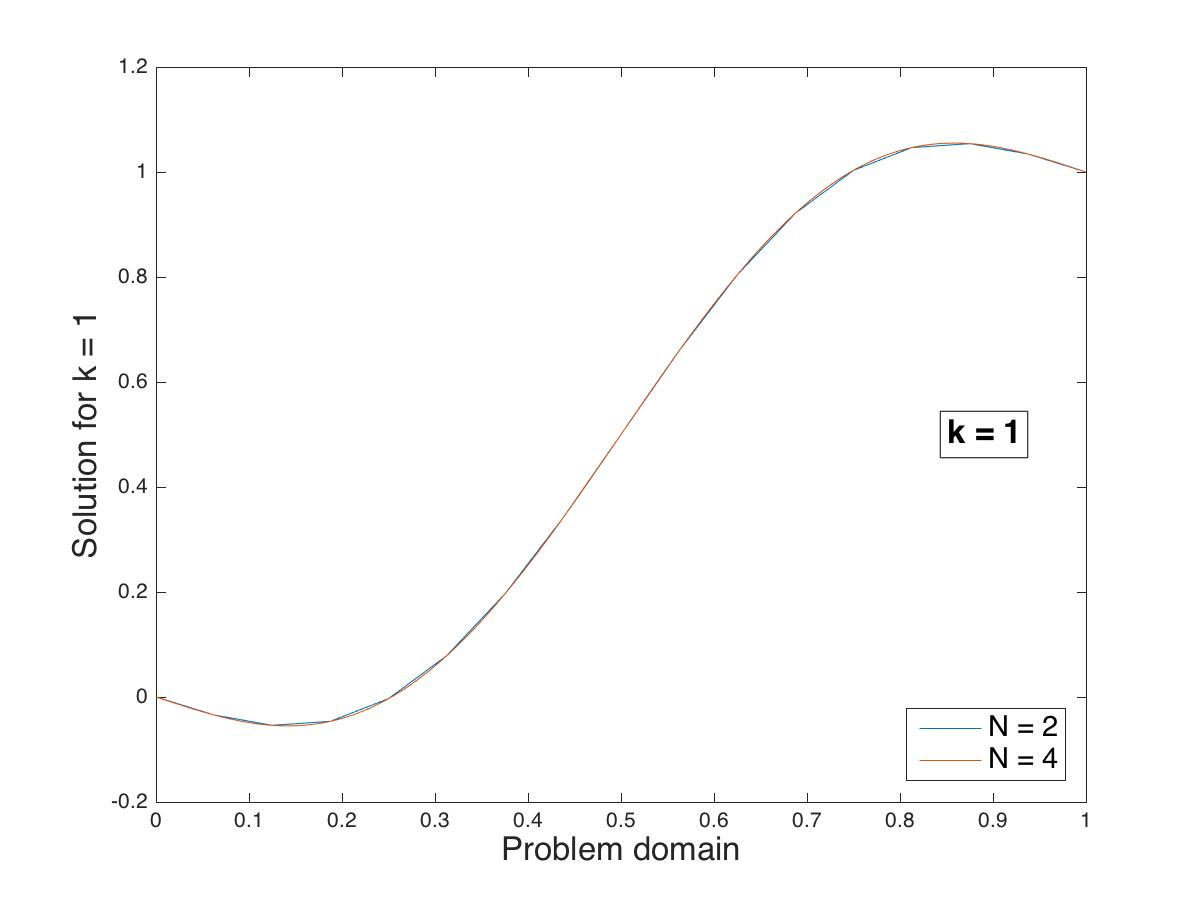
\includegraphics[width=1.0\linewidth]{Nplot_for_k_1.jpg}
  \caption{}
\end{subfigure}
\begin{subfigure}{.48\textwidth}
  \centering
  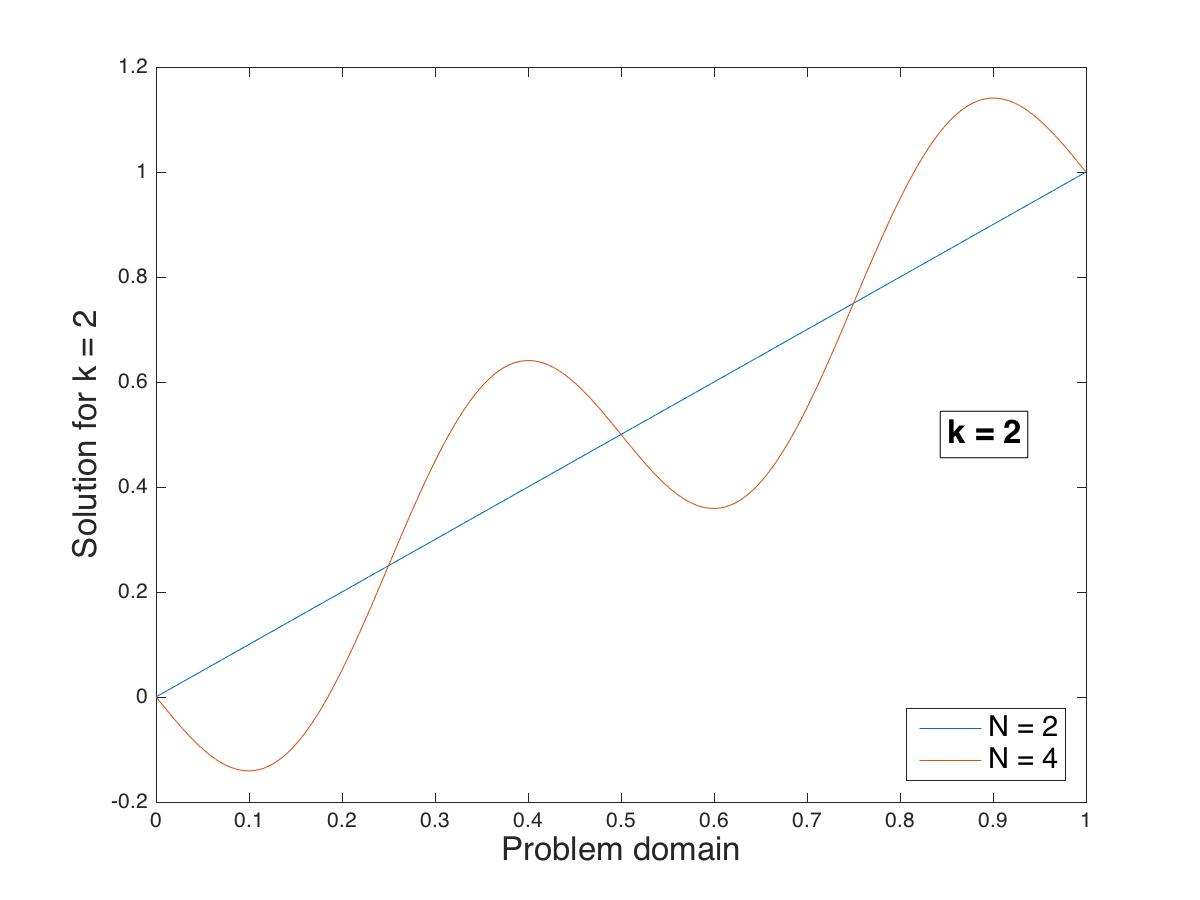
\includegraphics[width=1.0\linewidth]{Nplot_for_k_2.jpg}
  \caption{}
\end{subfigure}
\begin{subfigure}{.48\textwidth}
  \centering
  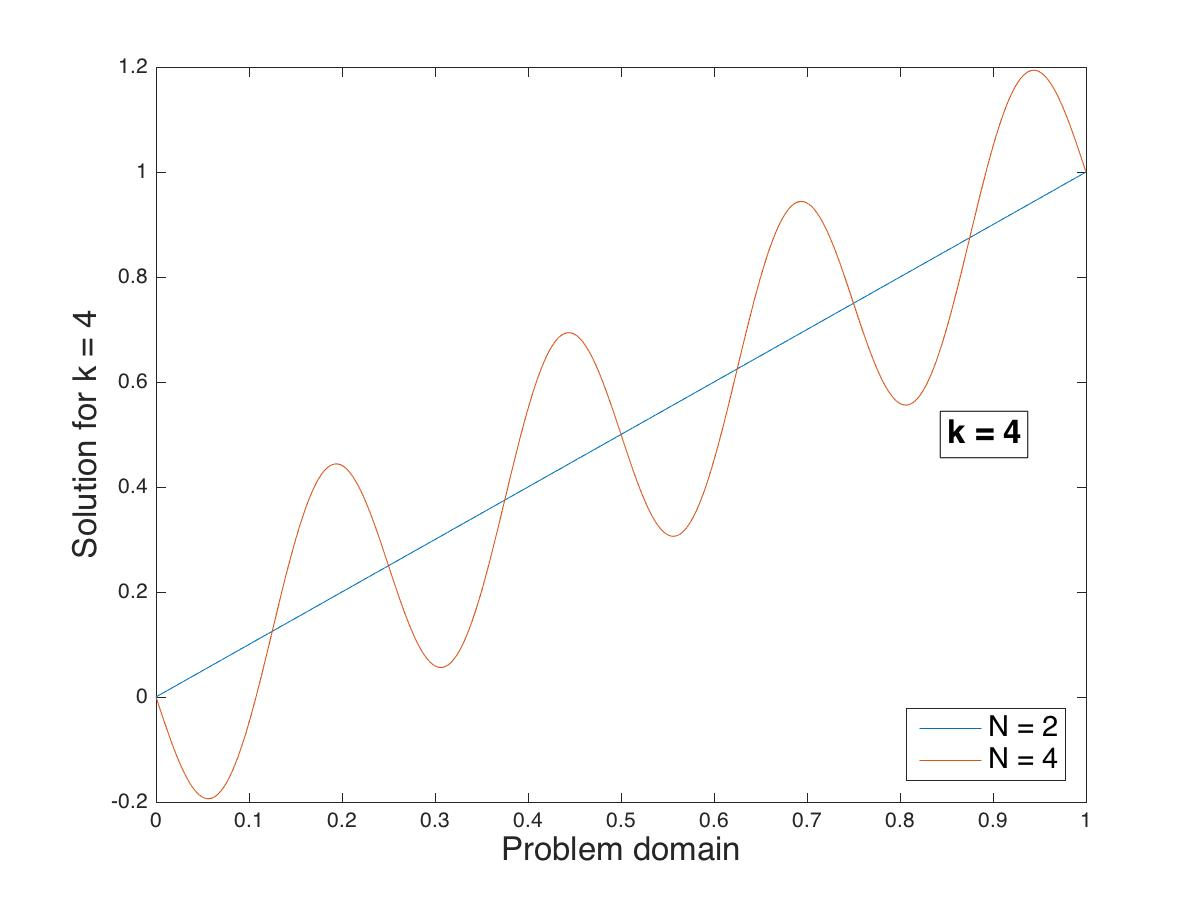
\includegraphics[width=1.0\linewidth]{Nplot_for_k_4.jpg}
  \caption{}
\end{subfigure}
\begin{subfigure}{.48\textwidth}
  \centering
  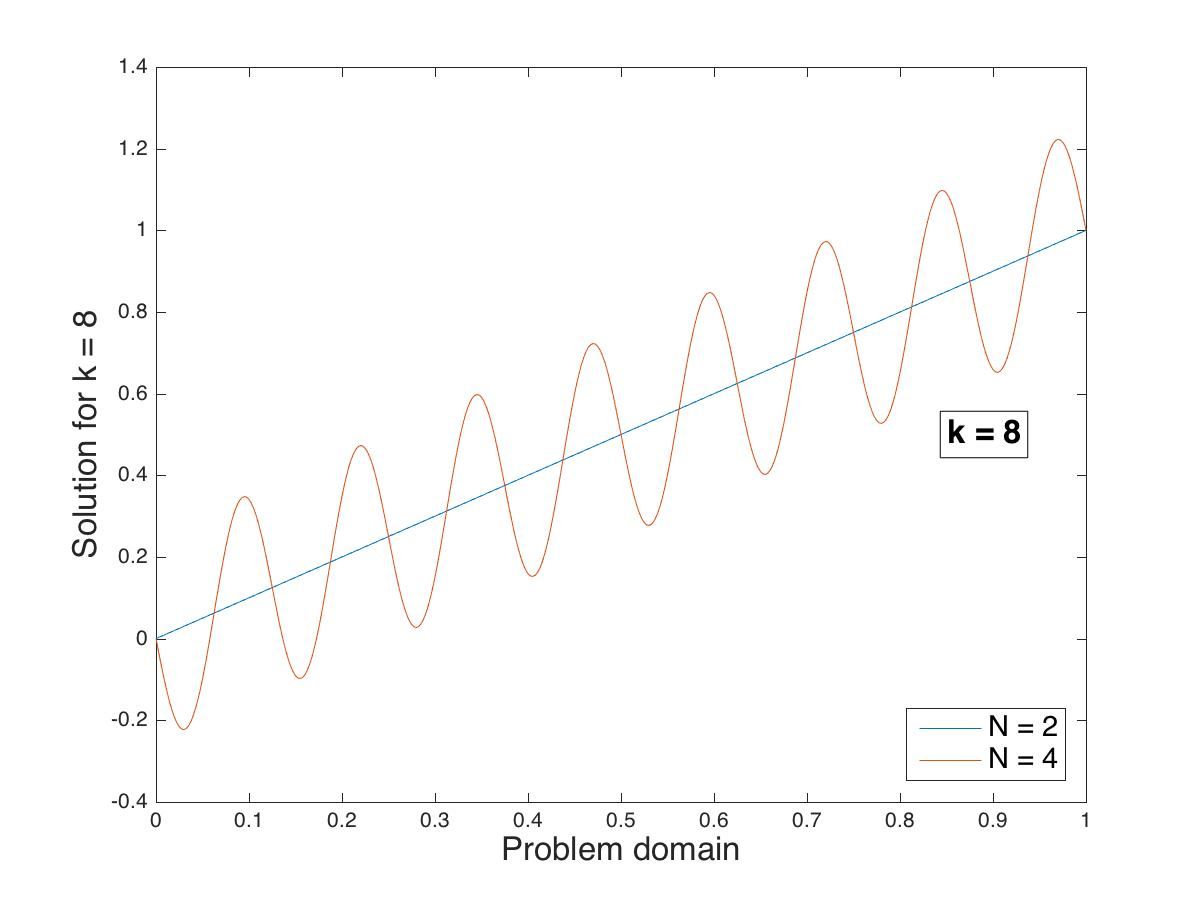
\includegraphics[width=1.0\linewidth]{Nplot_for_k_8.jpg}
  \caption{}
\end{subfigure}
\begin{subfigure}{.48\textwidth}
  \centering
  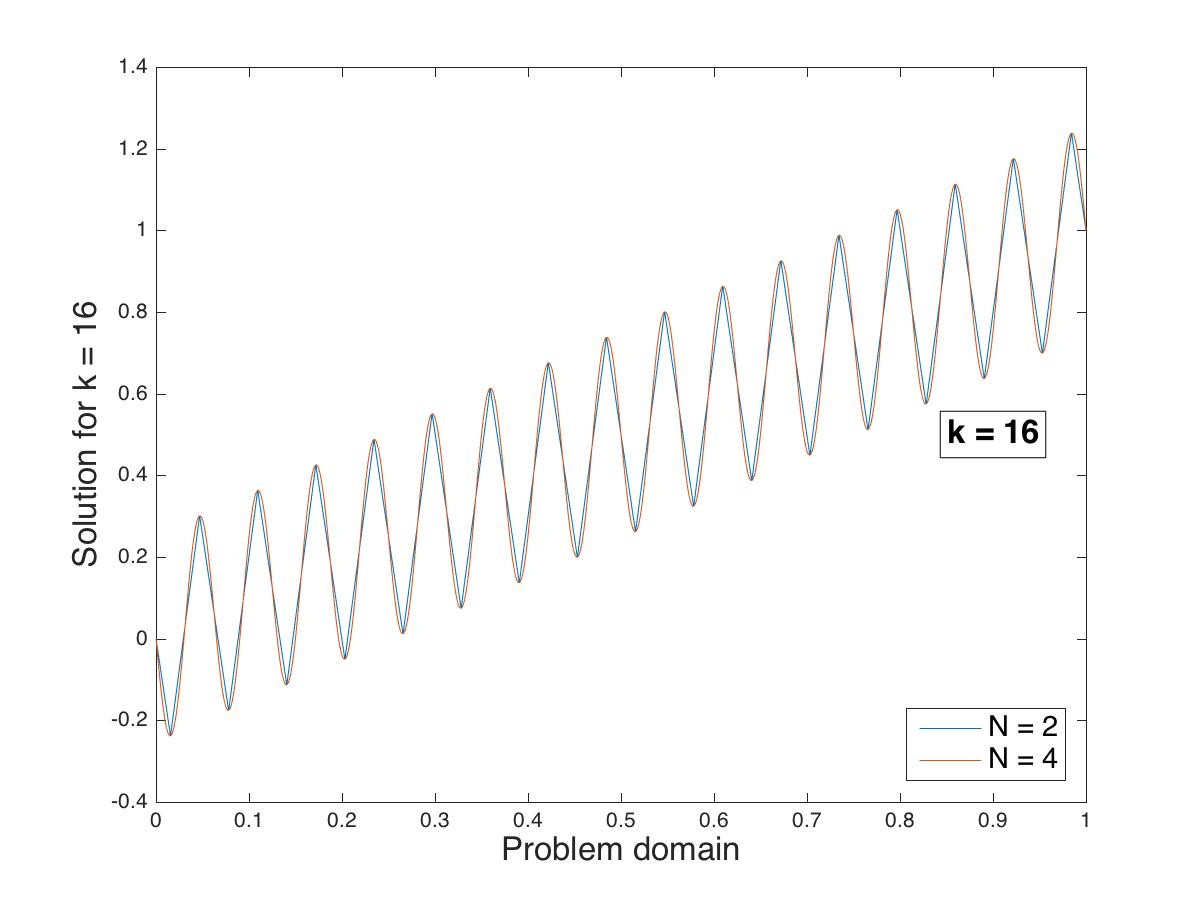
\includegraphics[width=1.0\linewidth]{Nplot_for_k_16.jpg}
  \caption{}
\end{subfigure}
\begin{subfigure}{.48\textwidth}
  \centering
  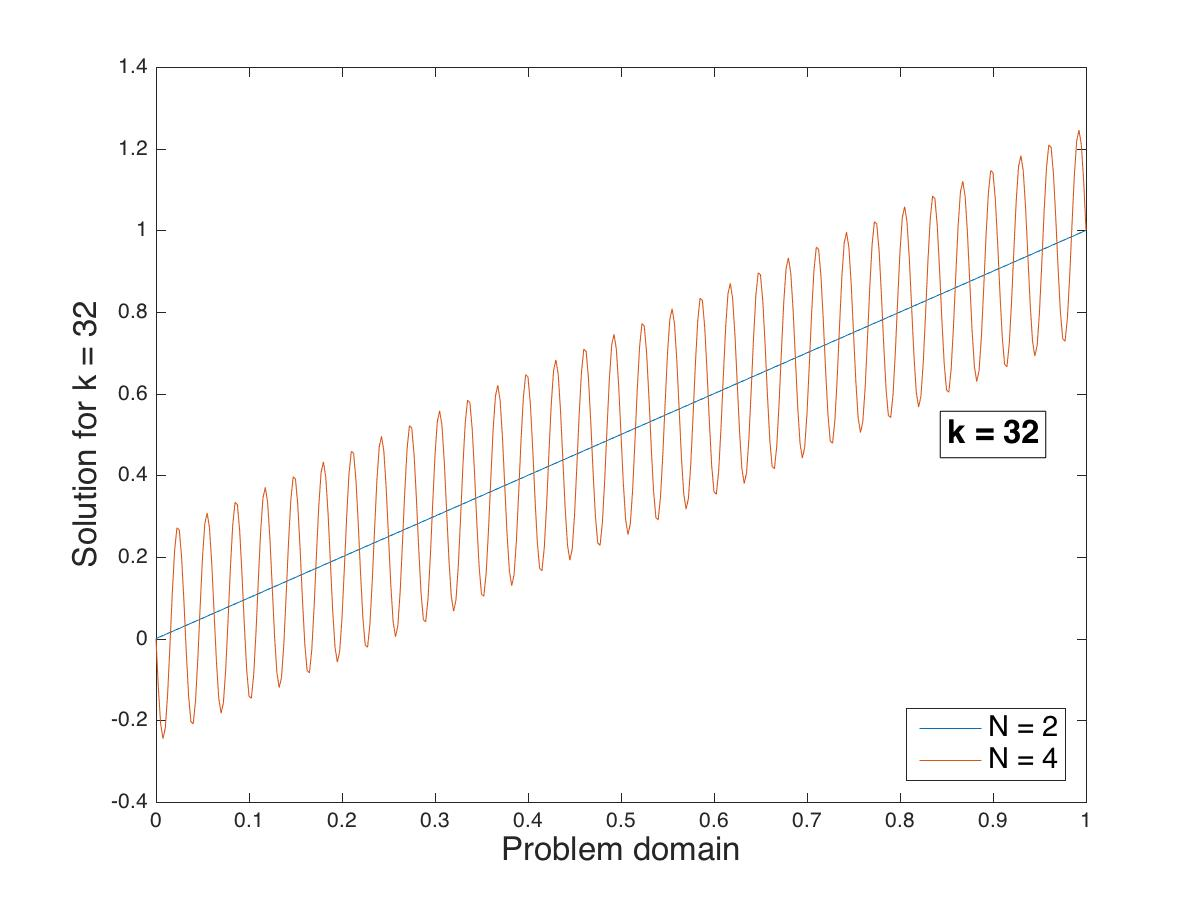
\includegraphics[width=1.0\linewidth]{Nplot_for_k_32.jpg}
  \caption{}
\end{subfigure}
\caption{Finite element and exact (analytical) solutions for \(N=2, 4, 8, 16, 32, 64, \) and \(128\) for (a) \(k=1\), (b) \(k=2\), (c) \(k=4\), (d) \(k=8\), (e) \(k=16\), and (f) \(k=32\).}
\label{fig:Nplots}
\end{figure}

Fig. \ref{fig:eN} shows \(e^N\) as a function of \(N\) for each value of \(k\) represented in the previous figure. \(N\) is allowed to vary from 1 to 128 to obtain a fine-enough plot to observe the convergence behavior. As can be seen, the higher the \(k\), the more elements that are needed to obtain a desired global energy norm. For very oscillatory solutions, for coarser meshes, nodes may happen to consistently \textit{not} ``fall'' in the peaks and valleys of the solution, completely missing the oscillatory behavior. Hence, increasing the mesh resolution for oscillatory solutions with high frequency  does not always reduce the energy norm simply due to where the nodes may happen to lie. However, with a fine-enough mesh, by increasing the number of elements, the energy norm will monotonically decrease. 

\begin{figure}[H]
  \centering
  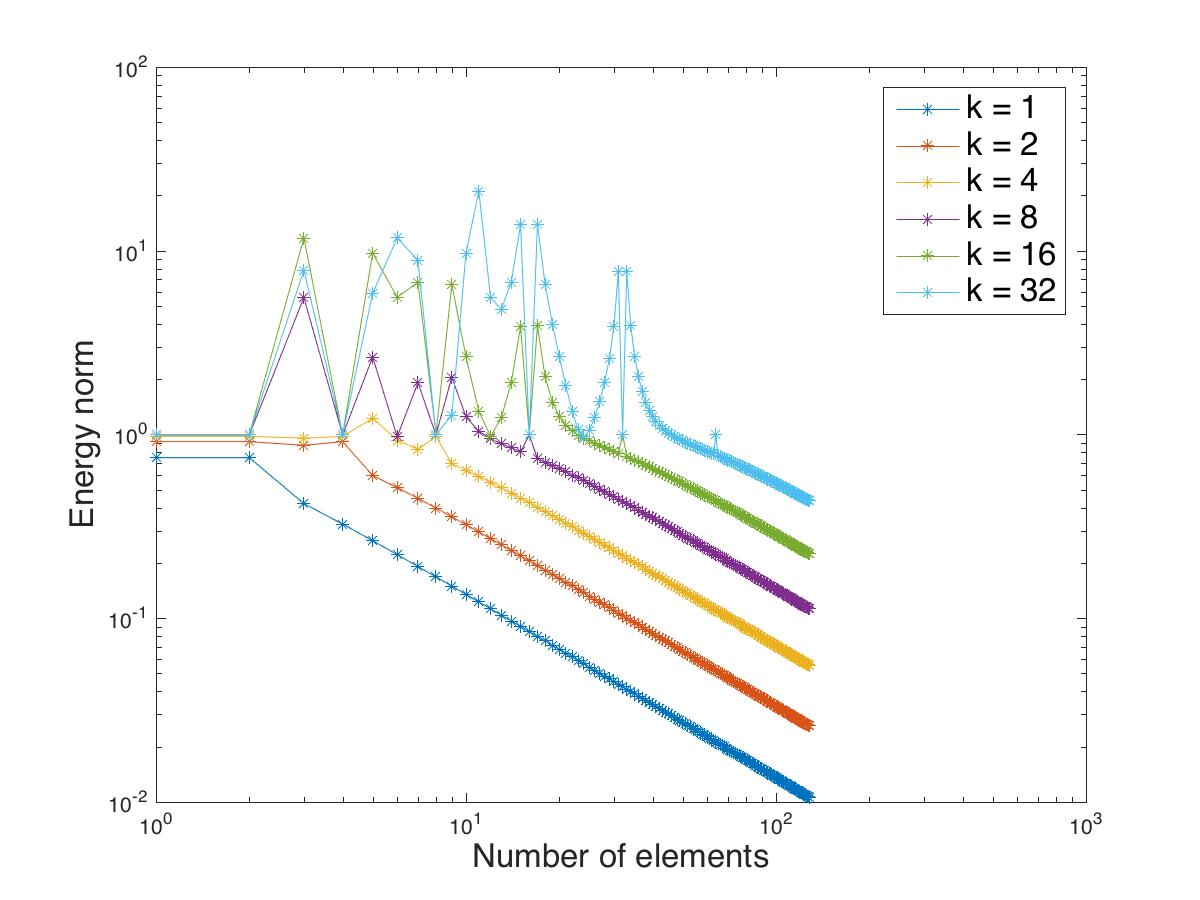
\includegraphics[width=13cm]{eN_vs_N.jpg}
  \caption{Energy norm \(e^N\) as a function of \(N\) for \(k=1, 2, 4, 8, 16, \) and \(32\).}
  \label{fig:eN}
\end{figure}

\section{Appendix}

This section contains the code used for this modeling. The main program is \texttt{FEProgram.m}, and functions perform specialized tasks for a high degree of modularity.

\subsection{\texttt{FEProgram.m}}
\lstinputlisting[language=Matlab]{FEProgram.m}

\subsection{\texttt{permutation.m}}
This function determines the permutation matrix for use with the connectivity matrix.
\lstinputlisting[language=Matlab]{permutation.m}

\subsection{\texttt{mesh.m}}
This function performs the meshing.
\lstinputlisting[language=Matlab]{mesh.m}

\subsection{\texttt{BCnodes.m}}
This function applies boundary conditions.
\lstinputlisting[language=Matlab]{BCnodes.m}

\subsection{\texttt{shapefunctions.m}}
This function contains the library of shape functions.
\lstinputlisting[language=Matlab]{shapefunctions.m}

\subsection{\texttt{quadrature.m}}
This function selects the quadrature rule.
\lstinputlisting[language=Matlab]{quadrature.m}

\subsection{\texttt{condensation.m}}
This function separates out the matrix equation as in Eq. \eqref{eq:condensation}.
\lstinputlisting[language=Matlab]{condensation.m}

\subsection{\texttt{postprocess.m}}
This function postprocesses the FE solution and transforms it back to the physical domain using a linear system solve as described in Eq. \eqref{eq:LinearSolve}.
\lstinputlisting[language=Matlab]{postprocess.m}


\end{document}